% ---- ETD Document Class and Useful Packages ---- %
\documentclass{ucetd}
\usepackage{subfigure,epsfig,amsfonts}
\usepackage{natbib}
\usepackage{amsmath}
\usepackage{amssymb}
\usepackage{amsthm}
\usepackage[toc,page]{appendix}
\usepackage[labelfont=bf]{caption}
\usepackage{rotating}

\usepackage{url}
 

%% Use these commands to set biographic information for the title page:
\title{Stochastic computation in recurrent networks of spiking neurons}
\author{Clayton W. Seitz}
\department{Graduate Program in Biophysics}
\division{Physical and Biological Sciences}
\degree{Master of Science}
\date{Winter 2021}

%% Use these commands to set a dedication and epigraph text

\epigraph{Epigraph}

\begin{document}
%% Basic setup commands
% If you don't want a title page comment out the next line and uncomment the line after it:
\maketitle
%\omittitle

% These lines can be commented out to disable the copyright/dedication/epigraph pages
\makecopyright
%\makededication
\makeepigraph


%% Make the various tables of contents
\tableofcontents
%\listoffigures
%\listoftables

\acknowledgments
% Enter Acknowledgements here

\abstract

The primate cerebral cortex is a complex system estimated to harbor more than 25 billion neurons communicating via action potentials or `spikes' and is responsible for many higher-order brain functions including memory and learning. Recent years have hosted many efforts to understand how such complex phenomena emerge from the communication of individual cells. Many studies have provided evidence that long term plasticity (LTP) in synapses permits a long-lasting alteration of network dynamics and, in turn, forms the basis of long-term memory and learning. However, understanding memory formation and learning in the brain is made difficult by the variability in the response of cortical neurons to stimuli. Therefore, capturing the apparent stochastic features of neural activity in computer based models, such as recurrent spiking neural networks (RSNNs), while explaining their manipulation of information mathematically has become the gold standard for computational neuroscience. Models of neural networks derived from statistical mechanics, such as those which assert that the membrane potential of a cortical neuron obeys a form of Langevin dynamics, can potentially account for stochastic network activity. Such models also provide the intriguing interpretation that neural activity represents sampling from a probability distribution - a technique central to statistical inference.  Here, we apply a similiar mathematical treatment to the study of an RSNN by modeling the membrane potential statistics of an integrate and fire neuron using Fokker-Planck equations. With this statistical framework in hand, we can recast a network of neurons as a stochastic process in higher dimensions and explore the relationships between synaptic connectivity and its plasticity to the correlation structure of neural spike trains. This approach is also amenable to information theoretic analysis and is a step toward a mathematical relationship between neuroplasticity mechanisms and the emergent computational capabilities of cortical microcircuits.



\mainmatter

\chapter{Stochastic computation in recurrent networks of spiking neurons}

\section{Introduction}

Complex systems are ubiquitous in nature yet our scientific efforts have thus far only begun to gain traction on their governing principles. Many of the most intriguing complex systems in nature exihibit behaviors that simply cannot be explained by any of the components in isolation but rather arise from their interactions, bringing emergent phenomena into the focus of modern science. The human cerebral cortex exemplifies this complexity, thought to consist of over 16 billion noisy nerve cells. However, the dynamics of neurons in cortex simulataneously maintain an order evident in the stability of our sensory percepts.

It is well accepted that information processing in the brain like sensory, motor, and cognitive functions are carried out by the communication between individual nerve cells, formally referred to as a \emph{population code}. Amongst a wide variety of cell types, the dominating information processing unit in neocortex is the spiking neuron - a  cell which exhibits transient depolarization and repolarization of the plasma membrane called action potentials or \emph{spikes}.  Neurons in cortex connect when afferent nerve fibers of one cell meet the dendritic tree or soma of another, forming the synapse. The complexity of the structure of neural networks therefore arises from the complex wiring of these communication channels. It is a great challenge to understand how connectivity patterns in cortex interact with sensory stimuli via synaptic transmission to give rise to conscious experience. 

In his famous neurophysiological postulate, Donald Hebb first proposed a cellular mechanism for the self-organization of networks of neurons. Hebb suggested that repeated stimulation of specific receptors of sensory signals would lead slowly to the formation of a \emph{cell assembly} and these structural changes would constitute a representation or imprint of an internally or externally generated sensation e.g., an image or idea [1]. This process, referred to as Hebbian learning, is argued to be driven by the temporal order of action potentials where the efficacy of transmission across a synapse can be modified according to sensory experience. Our understanding of these mechanisms from a neurobiological point view has drastically improved since this idea was first presented. However, phenomena which are thought to rely on changes in synaptic wiring, such as memory formation, still have yet to be fully explained from first principles.

At any rate, the computations carried out by cortical circuits cannot depend on synaptic wiring alone, but must depend on the dynamical constraints placed on networks of neurons by their biological constitution. Indeed, our understanding of such computations is greatly complicated by the introduction of realistic mechanisms for spike generation into our models. For example, depolarization of the neural membrane occurs via integration of post-synaptic potentials (PSPs) which in turn arise due to the release of synaptic vesicles containing excitatory or inhibitory neurotransmitters into the synaptic cleft. Furthermore, a host of dynamic plasticity mechanisms exist which are constantly modifying synaptic efficacy during the course of stimulation. Historically, these features of neural communication have been neglected in theoretical studies out of necessity. However, the lack of biological realism  does not necessarily preclude an improvement of our understanding of the computational paradigm employed by the brain. Even an extremely simplified model system, such as an ensemble of coupled binary units, can yield signficant insights into the mechanisms of neural computation (Hopfield, 1982). 

Furthermore, it stands to reason that the population code employed by cortical circuits will become evident after suitable analysis of the correlation structure of neural spike trains. Such correlations have been argued to originate in the overlapping synaptic input pools of two or more neurons (Rosenbaum 2017), which may result from synaptic plasticity. On the other hand, \emph{in-vivo}, spike-train correlations resulting from overlapping synaptic inputs must be distinguished from  correlations which arise from environmental factors outside a controlled stimulus. Often referred to as noise correlations, these correlations cannot be reproduced across experimental trials and are closely linked to the trail-to-trial variability observed experimentally. The role of noise correlations in the brain is poorly understood, although it is widely regarded to contribute to the amount of information that can be encoded by a neuronal population (Cohen 2011). In principle, stochasticity can be introduced into a system of neurons in a few different ways: (i) by intrinsic noise - the noise introduced into the system by the random interactions of a cell's molecular components at nonzero temperature (ii) background activity i.e., afferent synaptic inputs that are not members of the population being simulated or recorded (iii) by stochastic features of the stimulus used to generate network activity. If the system is assumed to be closed (as in a computer simulation), the only possible noise sources come from (i) and (iii). Therefore, in the remainder of the text, we assume that the only contributing factors to spike-train correlations are overlapping synaptic input pools and that any noise that is intrinsic to any one neuron is uncorrelated with that of all other neurons in the population.


An ideal theory of cortical dynamics would be able to precisely predict the future state of the state variables of each individual neuron, e.g. the membrane potential, given their current state. However, stochastic features of single neuron dynamics make such a theory intractable. Accordingly, some of the most mature models of cortical dynamics owe their origins to statistical physics. It is common in statistical physics to be faced with a very high-dimensional system whose microscopic dynamics cannot be predicted exactly. One solution to this problem is to develop a so-called mean field theory (MFT), where the interactions between individual units are replaced by their average values. While an approximation, this solution has had success in predicting the average dynamics of networks in the limit of very large numbers of neurons. Another approach is to develop an ensemble density model, where, under the appropriate assumptions, the probability density of neuron state variables and its dependence on time can be predicted analytically (Brunel 2000). Such models often rely on a diffusion approximation of the Kramers-Moyal expansion, which therefore involes the solution of a second-order differential equation for the population density of a state variable as a function of time. These equations are notoriously difficult to solve, although in a few special cases, a solution can be found.

Moreover, early models of cortical computation were deterministic and therefore assumed cortical computations are carried out in a logical fashion. However, an increasing body of experimental data suggests that neurons, synapses, and systems of neurons are inherently stochastic (Buesing, 2011). The enormous number of degrees of freedom of just a single cell due to millions of unreliable ion channels and synaptic machinery demands a stochastic model for network dynamics (Cannon, 2010; Tuckwell, 1989). Indeed, it has been argued that the trial-to-trial variability in neural responses to stimuli and the irregularity of spike-timing owe their origins to noise in the synaptic integration process (Azouz, 1999). Importantly, \emph{noise} here refers to unpredictable features of synaptic integration by the postsynaptic cell and not to the presynaptic spikes themselves. 

The apparent reliability of cortical computations at the scale of networks suggests that the brain has evolved to accomodate for synaptic noise or perhaps even incorporated the noise into its computational paradigm (Rolls, 2010). In recent decades, a great deal of effort has been spent investigating the hypothesis that networks of neurons perform sensory processing via probabilistic, rather than logical inference. Probabilistic inference is a rich mathematical framework that has experienced success in fields such as machine learning and artificial integlligence and, more recently, computational neuroscience. These ideas have been recently applied in a variety of subdomains including sensorimotor learning (Kording, 2004), object recognition (Kersten 2004), visual processing (Lee 2003), and perceptual multistability (Sundareswara 2008). In the probabilistic framework, neural responses to stimuli are viewed as sampling from a posterior distribution, conditioned on the stimulus (Hoyer 2002; Buesing 2011). This framework naturally accomodates for the stochastic effects introduced by the biological substrate. At the same time, a stochastic description of network dynamics does not exclude a rigorous understanding of the transmission of information. Quite the contrary, information transmission in single neurons can be quantified precisely via the use of Shannon's information theory (MacKay, McCulloch 1952). More recently, this theory has been applied in the quantification of how much information flows through the nervous system, and the constraints that information theory imposes on the capabilities of neural systems for communication, computation and behavior (Dimitrov 2011).

Most recently, artificial spiking neural networks (SNNs) have been developed that strive to replicate human cognitive capabilities such as language processing or temporal credit assignment (Bellec 2020). Such networks incorporate biologically plausible online learning rules thought to be similar to those employed by the brain.
Nevertheless, these models are highly task-oriented and therefore difficult to apply to other tasks or sensory processing at large. Therefore, here we consider the dynamics of a spiking neural network stimulated with a multivariate gaussian signal with well-defined covariance. 


\section{Theory}

A central goal of modern neuroscience is to explain how functional brain states emerge from the interactions of dozens, perhaps hundreds, of brain regions, each containing its own complex subnetworks.  These subnetworks can themselves contain thousands of cells, each neuron having on the order of thousands of synaptic connections to other cells within the local network (Binzegger 2004). In fact, connection probabilities between nearby neurons in cortex has been shown experimentally to sometimes exceed 40 percent (Ko 2011; Levy 2012) suggesting a \emph{small-world} organization of the brain. 

The canonical small-world network developed by Watts and Strogatz is one in which the majority of connections form small densely connected clusters with respect to the size of larger brain regions.  The remaining connections then maintain intermediate connections between these islands of dense synaptic connectivity. The conjunction of local clustering and global interaction provides a structural substrate for the coexistence of functional segregation and integration in the brain (Sporns 2006). Also, this structural quality of brain networks has led to network models which consist of large numbers of densely connected populations with sparse channels of connectivity between them, called fractal networks (Sporns 2006).


\subsection{The uncorrelated regime}

Dynamical network models that incorporate this kind of spatial information present a challenge for theoretical calculations of population dynamics. This has led to the description of neural field theories or tissue scale models which provide a coarse-grained description of cortical activity, such as population-scale fluctuations in the firing rate. Moving towards a more fine description of network dynamics, some have assumed a small number of discrete populations of cells - a classic example being the excitatory inhibitory random network. For example, population density methods have been used to succesfully predict the steady-state firing rates and membrane potential density of the excitatory-inhibitory random network using the Fokker-Planck formalism (Brunel 2000). Consider the following ordinary differential equation for the membrane potential of a neuron $j$

\begin{equation}
\tau\dot{V_{j}}(t) = -V_{j}(t) + I_{j}(t)
\end{equation}

which is a Langevin equation. Take the case when $I_{j}(t)$ is the post-synaptic potential induced by feedforward and recurrent synaptic currents plus additive noise

\begin{align}
I_{j}(t) = F_{j}(t) + R_{j}(t) + \sigma_{j}\sqrt{dt}\eta(t)
\end{align}

where we have reserved $\eta(t) \sim \mathcal{N}(0,1)$ for the intrinsic noise of a neuron. We assume that this intrinsic noise is delta correlated i.e. $\langle \eta_{i}(t)\eta_{j}(t)\rangle = \delta(i-j)$ and $\langle \eta_{i}(t)\eta_{i}(t+\tau)\rangle = \delta(\tau)$. Obviously, the same condition is not necessarily satisifed for the total synaptic current: there exist network architectures and stimulus regimes that can realize a case where $\langle I_{i}(t)I_{j}(t)\rangle \neq 0$ and $\langle I_{i}(t)I_{i}(t+\tau)\rangle \neq 0$ for $i \neq j$.


There are several  ways in which pairwise correlations can vanish. One is if the network topology is sufficiently sparse that it is unlikely that two neurons share common inputs or synaptic weights are sufficiently small that the timing of a spike is driven by intrinsic noise, which is often assumed to be uncorrelated between neurons (Plesser 2000). Another is when the network is balanced in such a way that uncorrelated inputs cause the total correlation to become weak (Rosenbaum 2017). The first condition was used to derive an expression for the steady state population voltage distribution using the Fokker-Planck equation (Brunel 2000), an extension of previous work where an expression for the steady-state firing rate was derived analytically (Riccardi 1977; Amit 1991). If any of the criteria for uncorrelated synaptic inputs are met, the post-synaptic potentials in (1.7) will have a normal distribution according to the central limit theorem.


%\clearpage
\begin{figure}[t!]
\centering
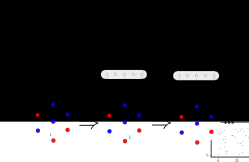
\includegraphics[width=150mm]{figure-1}
\caption{(a) Diagram of a recurrent neural network receving a time-dependent feedforward stimulus. (b) Diagram of the stochastic encoding scheme used a recurrent neural network with noise}
\end{figure}

Uncorrelated synaptic currents greatly simplify the analysis of network dynamics. The previously $N$-dimensional stochastic differential equation for the voltage can be collapsed to one dimension and the problem becomes the determination of the voltage density over the population (or for a single neuron) $P(V,t)$. This can be done by making use of the Kramers-Moyal expansion, which is derived from the Chapman-Kolmogorov (CK) equation

\begin{equation}
P(V'_{j}, t) = \int T_{j}(V'_{j}, t | V_{j}, t-\tau)P(V_{j}, t-\tau)dV
\end{equation} 

In words, the voltage distribution at a time $t$ is expressed as an integral over all possible previous states $P(V_{j}, t-\tau)$ and the probability of transition $T_{j}(V'_{j}, t | V_{j})$ or \emph{transition operator}. From the above equation we can derive the Kramers-Moyal Expansion (KME) which has the form

\begin{align}
\frac{\partial P_{j}}{\partial t} = \sum_{n} \frac{(-1)^{n}}{n!} \left(\frac{\partial}{\partial V_{j}}\right)^{n} M_{n}(V_{j},t,\tau) P(V_{j},t)
\end{align}

where $M_{n}(V,t,\tau)$ denotes the $nth$ order moment of the transition density $T_{j}(V'_{j}, t | V_{j}, t-\tau)$. If we approximate the KME by truncating the summation for $n > 2$ we arrive at the so-called \emph{diffusion approximation} or Fokker-Planck equation

\begin{align}
\frac{\partial P_{j}(V,t)}{\partial t} &= \frac{\partial}{\partial V_{j}}[\left(V_{j}(t)-\mu_{j}(t)\right) P_{j}(V_{j},t)] + \frac{\sigma_{j}^{2}(t)}{2}\frac{\partial^{2}}{\partial V_{j}^{2}}[P(V_{j},t)]
\end{align}

More recent developments have relied on a mean-field theory of neuronal interactions in large populations. This approach appears promising for its account of the stochastic features of network dynamics while maintaining a description of population dynamics with resolution down to the individual neuron. It is also readily applicable to populations with small-world features and even networks with connection probabilities defined continuously over a spatial domain (Rosenbaum 2017).

Neurons in cortex are characterized by irregular time intervals between spikes. However, the role of this temporal irregularity in sensory processing remains unclear. One hypothesis that attempts to explain this irregularity claims that an approximate balance of excitatory and inhibitory synaptic currents explains the large coefficient of variation observed in cortex (Vreeswijk, 1996). In this balanced regime, the timing of the firing of cells in cortex is sensitive to the relatively small fluctuations in their total synaptic input because the excitatory and inhibitory inputs cancel each other (Amit, 1995). Also, excitatory and inhibitory balance has been theoretically shown to enhance the sensitivity of fast stimulus fluctuations much smaller than a typical integration time constant for a single neuron (Vreeswijk, 1996; Tian 2020). Interestingly, model neurons optimally detect temporal information when the average membrane potential is one standard deviation of the noise below threshold, a phenomenon known as stochastic resonance (Plesser, 2000; Kempter, 1998).

Furthermore, the complexity of cortical networks and subnetworks therein present very large parameter spaces for analytical study and computer simulations. Exploring this parameter space exhaustively is extremely computationally expensive, demanding the careful choice of our origin within such a space. If the network model contains both excitatory and inhibitory neurons, a natural starting point is one in which excitatory, inhibitory, and feedforward currents balance each other (Vreeswijk, 1996). Indeed, one can construct a newtork in which this occurs by using a mean-field theory of synaptic currents into single neurons embedded in a large population. In the following paragraphs, the terminology and mathematical machinery needed to build this network will be described.


A network model is called \emph{sparse} if the probability of a connection between a neuron in a population $\alpha$ and another neurons in a population $\beta$ scales with the network size $N$ according to $p_{\alpha\beta} \sim \mathcal{O}(1/N)$. Using terminology borrowed from graph theory, the degree $K$ of a neuron does not depend on the scale of the network or $K \sim \mathcal{O}(1)$. In contrast, we then say that a network is \emph{dense} if the above connection probability scales as $p_{\alpha\beta} \sim \mathcal{O}(1)$ such that the degree of a neuron scales as $K \sim \mathcal{O}(N)$. Moreover, the efficacy of a synaptic connection between populations $\alpha$ and $\beta$ is said to be \emph{strong} if $J_{\alpha\beta} \sim \mathcal{O}(1)$ and \emph{weak} coupling occurs when $J_{\alpha\beta} \sim \mathcal{O}(1/\sqrt{N})$. This choice of scaling for $J_{\alpha\beta}$ and the degree $K$ results in the total synaptic input to a neuron scaling as $\mathcal{O}(\sqrt{N})$. In this case, it is possible parameterize the network s.t. fluctuations in the synaptic input currents saturates to a value of the order of the spiking threshold, in the limit of large $N$ (Vreeswijk, 1996; Renart 2010; Rosenbaum 2017).  

The scaling of synaptic inputs outline above are a critical step towards finding the balanced state. To see this, consider the total synaptic current injected into a neuron $i$ within a population $\alpha$, decomposed into its feedfoward and recurrent components

\begin{align}
I_{i}^{\alpha}(t) &= F_{i}^{\alpha}(t) + R_{i}^{\alpha}(t)\\
&= F_{i}^{\alpha}(t) + \sum_{\beta}\sum_{j} \frac{J_{ij}^{\alpha\beta}}{\sqrt{N}}(\psi * z^{\beta}_{j}(t))
\end{align}

where the variable $z^{\beta}_{j}(t)$ is sometimes called the \emph{observable state} of neuron $j$ and is given by thresholding the voltage: $z^{\beta}_{j}(t) = H(v^{\beta}_{j}(t) - \theta)$ where $H$ is the Heaviside step function. For the sake of generality, the term $z^{\beta}_{j}(t)$ is convolved with a with a kernel $\psi$, determining the shape of the post-synaptic potential induced by a spike. In the mean-field approximation we replace the current in each term of the sum over $j$ in (1.2) by its average value, which is a valid approximation in the limit $N\rightarrow\infty$ (Vreeswijk 1996). Taking $\psi = \delta(t)$, the observable state $z^{\beta}_{j}(t)$ is replaced by the average firing rate of a neuron in population $\beta$ multiplied by the probability of a connection $p_{\alpha\beta}$

\begin{align*}
\langle I_{i}^{\alpha}(t)\rangle &= \langle F_{i}^{\alpha}(t)\rangle + \langle R_{i}^{\alpha}(t)\rangle\\
&= \langle F_{i}^{\alpha}(t)\rangle + \sqrt{N}\sum_{\beta}j_{\alpha\beta}p_{\alpha\beta}r_{\beta}
\end{align*}

with $j_{\alpha\beta} = J_{\alpha\beta}\sqrt{N}$. Notice that the average value of the recurrent contribution to the synaptic current indeed saturates for large $N$. Writing the above equation explicitly for a neuron in an excitatory-inhibitory network i.e. $\alpha, \beta \in \{e, i\}$

\begin{align}
\langle I_{j}^{e}(t)\rangle &= \langle F_{j}^{e}(t)\rangle + \sqrt{N}\left(j_{ee}p_{ee}r_{e} + j_{ie}p_{ie}r_{i}\right)\\
\langle I_{k}^{i}(t)\rangle &= \langle F_{k}^{i}(t)\rangle + \sqrt{N}\left(j_{ii}p_{ii}r_{i} + j_{ei}p_{ei}r_{e}\right)
\end{align}

If we require that, in the mean-field limit $N\rightarrow\infty$, the average current vanishes and that $\langle F_{j}^{\alpha}(t)\rangle \sim \mathcal{O}(\sqrt{N})$ we have the following matrix equation relating the mean field firing rates to the synaptic weights and average feedforward current

\begin{align}
\begin{pmatrix}
j_{ee} & j_{ie}\\
j_{ei} & j_{ii}
\end{pmatrix}
\begin{pmatrix}
r_{e}\\
r_{i}
\end{pmatrix}
= 
-\begin{pmatrix}
\langle F_{j}^{e}\rangle\\
\langle F_{k}^{i}\rangle
\end{pmatrix}
\end{align}

which can be summarized as $\mathbf{r} = -\mathbf{J}^{-1}\mathbf{f}$. Assuming that $\mathbf{J}$ is invertible, we have the following solution

\begin{align}
\underset{N\rightarrow \infty}{\mathrm{lim}}r_{e} = \frac{\langle F_{j}^{e}\rangle j_{ii}-\langle F_{k}^{i}\rangle j_{ie}}{j_{ei}j_{ie} - j_{ee}j_{ii}}
\end{align}

\begin{align}
\underset{N\rightarrow \infty}{\mathrm{lim}}r_{i} = \frac{\langle F_{k}^{i}\rangle j_{ee}-\langle F_{j}^{e}\rangle j_{ei}}{j_{ei}j_{ie} - j_{ee}j_{ii}}
\end{align}

For positive solutions for the above firing rates and for the above matrix to be invertible we have the rather loose condition $\langle F_{j}^{e}\rangle/\langle F_{k}^{i}\rangle > j_{ie}/j_{ii} > j_{ee}/j_{ei}$ and we recover the condition given in (Rosenbaum 2014; Rosenbaum 2017; Akil 2021). 

Since the balanced state is simultaneously an asychronous state, the recurrent inputs $R_{i}$ are uncorrelated and can be written as a gaussian random variable

\begin{align*}
R_{i}(t) = \sqrt{N}\mu_{R}(t) + \sigma_{R}(t)\xi_{R}(t)
\end{align*}

where $\mu_{R}^{\alpha} = (j_{e\alpha}p_{e\alpha}r_{e\alpha} + j_{i\alpha}p_{i\alpha}r_{e\alpha})$ and $\sigma_{R}^{\alpha} = (j_{e\alpha}^{2}p_{e\alpha}r_{e\alpha} + j_{i\alpha}^{2}p_{i\alpha}r_{e\alpha})$ (Brunel 2000).


Assuming the feedforward current $F_{i}(t)$ is also uncorrelated, the total current is also a gaussian random variable 

\begin{align*}
I_{i}(t) = \sqrt{N}\mu_{I}(t) + \sigma_{R}(t)\xi_{R}(t)
\end{align*}


using the shorthand $\mu_{I}(t) = \mu_{F}(t) + \mu_{R}(t)$ and $\sigma_{I}(t) = \sigma_{F}(t) + \sigma_{R}(t)$. The Fokker-Planck equation in (1.5) then applies, and becomes

\begin{align}
\frac{\partial P(V,t)}{\partial t} &= \frac{\partial}{\partial V}[\left(V(t)-\mu_{I}(t)\right) P(V,t)] + \frac{\sigma_{I}^{2}(t)}{2}\frac{\partial^{2}}{\partial V^{2}}[P(V,t)]
\end{align}

Due to the firing threshold $\theta$, boundary conditions on the above equation must be imposed (Brunel and Hakim 1999; Brunel 2000)

\begin{align*}
P(V,t) &= 0, v\geq \theta\\
P(v_{r}^{-},t) &= P(v_{r}^{+})\\
\frac{\partial P(v_{r}^{+},t)}{\partial t}-\frac{\partial P(v_{r}^{-},t)}{\partial t} &= \frac{\partial P(\theta,t)}{\partial t}\\
\int_{-\infty}^{\theta} P(V,t)dV &= 1
\end{align*}


\subsection{The correlated regime}

Recent studies have strongly suggested that understanding the neural code will amount to a rigorous understanding of correlations between neuron spike-timing. Such correlation studies are necessarily contextual - correlations must be interpeted in the context of known stimulus drive, learning or experience, or changes in behavioral context (Cohen 2011). This presents a significant challenge for theoretical studies given that the correlation structure of spiking between neurons can be considered a highly granular description of the population dynamics.

In the correlated regime, (1.10) no longer applies. Solving (1.10) in higher dimensions is difficult, and the use of Monte Carlo simulations requires a sample size that increses at an exponential rate, not to mention the associated computational costs. In addition, traditional numerical methods such as finite element and finite difference all suffer from the curse of dimension (Chen 2017, Pichler 2013). However, recently a method for solving the Fokker-Planck equation in high dimensions, even on the order of millions, has been developed for networks of Fitzhugh-Nagumo neurons with non-Gaussian features (Chen 2017), which may be a viable option in the future.

In sensory systems, correlations can be separated into signal and noise components. The signal correlation refers to the correlation that is repeatable across trials when the stimulus is identical. On the other hand, the noise correlation represents the component of the correlation that cannot be reproduced across trials. The role of noise correlations in the brain is poorly understood, although it is widely regarded to contribute to the amount of information that can be encoded by a neuronal population (Cohen 2011). It may be argued that noise correlations arise from hidden variables that are difficult to observe experimentally. In principle, stochasticity can be introduced into a system of neurons in a few different ways: (i) by intrinsic noise - the noise introduced into the system by the random interactions of a cell's molecular components at nonzero temperature (ii) background activity i.e., afferent synaptic inputs that are not members of the population being simulated or recorded (iii) by stochastic features of the stimulus used to generate network activity. If the system is assumed to be closed (as in a network simulation), the only possible noise sources come from (i) and (iii). In our remaining analysis, we assume the system is closed and that the only contributing factors to neuronal correlations are overlapping synaptic input pools and that any intrinsic noise is uncorrelated.

\subsection{Bayesian models of cognition}

\subsection{The neural sampling hypothesis}

\section{Results}


\begin{sidewaysfigure}
\centering

\includegraphics[scale=1.1]{figure-2}
\caption{Weak correlations of synaptic currents in the asychronous state}
\label{fig:foo}
\end{sidewaysfigure}



\subsection{The two-dimensional Gaussian network}

Suppose that we have a two-dimensional lattice which contains points separated by a distance $\Delta$ along the axial directions with periodic boundary conditions. The distance between any two points on such a lattice is the following Euclidean distance metric

\begin{align*}
|\Delta\mathbf{r}_{ij}|^{2} = \mathrm{min}(|x_1 - x_2|, n\Delta - |x_1 - x_2|)^2 + \mathrm{min}(|y_1 - y_2|, n\Delta - |y_1 - y_2|)^2
\end{align*}

Now, let the kernel $\Gamma_{ij}$ be the two-dimensional symmetric Gaussian

\begin{align}
\Gamma_{ij}(|\Delta\mathbf{r}_{ij}|) = \gamma\cdot \exp\left(-\frac{1}{2}(\mathbf{r}_{i}-\mathbf{r}_{j})^{T}\mathbf{\Sigma}_{i}(\mathbf{r}_{i}-\mathbf{r}_{j})\right)
\end{align}

where $\mathbf{\Sigma}_{i} = \sigma_{i}^{2}I$ with the two-dimesional identity matrix $I$. The parameter $\sigma_{i}$ can be intepreted as the \emph{reach} of a neuron $i$. Furthermore, for the kernel $\Gamma_{ij}$ to represent a binomial probability at each point of its domain, we must have that


\begin{equation}
\Gamma_{ij}(|\Delta\mathbf{r}_{ij}|)  \leq 1
\end{equation}

Plugging in our definition (3.5) gives the following inequality

\begin{align*}
\gamma\cdot \exp\left(-\frac{\underset{j}{\mathrm{min}}\left(|\Delta\mathbf{r}_{ij}|^{2}\right)}{2\sigma_{i}^{2}} \right) \leq 1
\end{align*}

The largest possible value of the exponential is achieved at $\underset{j}{\mathrm{min}}\left(|\Delta\mathbf{r}_{ij}|^{2}\right) = \Delta$ (a neighboring lattice point). Therefore, $\gamma$ is upper bounded according to $\gamma \leq \exp\left(\frac{\Delta^{2}}{2\sigma_{i}^{2}}\right)$. For the remainder of our analysis we will fix $\gamma = 1$ and focus our attention to the impact of the parameters $\sigma$ and $\Gamma_{0}$ on the statistics of connectivity. 

As can be seen in Fig. (3.1a), when $\Gamma_{ij} = \Gamma_{ji}$ we have that $p_{ij} = p_{ji}$ for all $|\Delta \mathbf{r}_{ij}|$. We formally refer to this case as the \emph{homogeneous gaussian network}. While this is not necessarily a realistic case, it serves as a useful testbed for the graph theoretic concepts to be used in later analyses. 

\begin{figure}[t!]
\centering
\includegraphics[width=100mm]{fig_11}
\caption{\textbf{Synapse probabilities for gaussian connectivity} (a) Binomial probabilities for two identical gaussian kernels ($\sigma=1$) separated by a distance $|\Delta\mathbf{r}_{ij}|$ and the probability of no synapse $\Gamma_{0}$ (left) and the corresponding multinomial probabilities (right). (b) Binomial probabilities for two different gaussian kernels ($\sigma_{1}=1, \sigma_{2}=2$) separated by a distance $|\Delta\mathbf{r}_{ij}|$ and the probability of no synapse $\Gamma_{0}$ (left) and the corresponding multinomial probabilities (right). }
\end{figure}



\subsection{Homogeneous Gaussian networks}

Let us now examine the statistics of the out-degree of a neuron $i$ assuming that the connectivity parameter $\sigma$ and $\Gamma_{0}$ are homogeneous across the network i.e., they are constant for all neurons. Using Eq. (3.2), we have

\begin{align}
\langle N_{ij} \rangle &= \left(\frac{1-\Gamma_{0}}{N}\right)\sum_{j} \Gamma_{ij}(1-\Gamma_{ji})\cdot Z_{ij}^{-1}
\end{align}

a sum that can be carried out numerically. Interestingly, in the homogeneous case, the parameter $\gamma$ and $\Gamma_{0}$ become redundant. This can be seen by considering that multiplying $p_{ij}$ and $p_{ji}$ by the same constant factor $\gamma$ is equivalent to the transformation $\Gamma_{0}' = 1-\gamma(1-\Gamma_{0})$. 

\begin{figure}[t!]
\centering
\includegraphics[width=175mm]{fig_8}
\caption{\textbf{The homogeneous Gaussian network}. (A) An example homogeneous network containing $N=100$ neurons. (B) An example neuron extracted from (A) with outgoing synapses labeled in blue and incoming synapses labeled in red. (C,D) The ratio $\langle N_{ij}\rangle/N$ as a function parameters ($\sigma, \Gamma_{0}$) for a sparse network (C) and a network with variable sparsity (D). (E,F) The ratio $\langle N_{ij}\rangle/N$ for fixed $\sigma$ and variable sparsity. (G,H) Binomial probability maps for two nearby neurons expressed as a sum $p_{ij}+p_{ji}$ and product $p_{ij}p_{ji}$}
\end{figure}

In other words, for the homogeneous case, the multiplication by $\gamma$ can be represented by a suitable selection of $\Gamma_{0}$ and can be set $\gamma=1$. Numerical evaluation of (3.7) shows that the ratio $\langle N_{ij}\rangle$ increases monotonically for increasing $\sigma$, as expected from (3.1b) and saturates at $\langle N_{ij}\rangle = 0.5$ at a rate proportional to $\sigma$. This can be understood from the fact that as $\Gamma_{0} \rightarrow 1$ we have $p_{0} \rightarrow 0$ and the multinomial distribution in (3.2) is reduced to a binomial distribution with $p_{ij} = p_{ji} = 1/2$. 

Furthermore, in addition to the average degree of a neuron, we are interested in the average number of shared inputs (outputs) between two neurons. We expect that this statistic makes at least a partial contribution to pairwise correlations in the voltage dynamics between two cells. To address this, we consider the average number of shared connections $\langle S_{ij} \rangle$ between a neuron $i$ and $j$ as a function of their distance $|\Delta \mathbf{r}_{ij}|$. In essence, this is the product $p_{ik}\cdot p_{jk}$ for a third neuron $k$ with $i,j\neq k$. The symmetry present in the homogeneous case allows us to perform this computation rather easily,

\begin{align}
\langle S_{ij} \rangle &= \frac{1}{N}\sum_{k} p_{ik}\cdot p_{jk} \\
&= \frac{\left(1-\Gamma_{0}\right)^{2}}{N}\sum_{k}\frac{\Gamma_{ik}(1-\Gamma_{ki})\Gamma_{jk}(1-\Gamma_{kj})}{Z_{ik}Z_{jk}}
\end{align}


which can be carried out numerically over the two-dimensions of space. Self-consistent with our definition of the connectivity kernel, the normalized number of shared connections decays with a gaussian profile for increasing $|\Delta \mathbf{r}_{ij}|$ as can be seen in Fig. (3.3).

\begin{figure}
\centering
\includegraphics[width=175mm]{fig_9}
\caption{\textbf{Shared connections in a homogeneous Gaussian network} (A,B,C) The average number of shared incoming or outgoing connections $\langle S_{ij}\rangle /N$ as a function of distance between two neurons $|\Delta r_{ij}|$ for three different values of the reach parameter $\sigma$.}
\end{figure}



\subsection{Excitatory-inhibitory Gaussian networks}

Thus far we have considered only the case where the spatial connectivity kernel is the same for every neuron. However, the integrative properties of neurons depend strongly on the number, proportions and distribution of excitatory and inhibitory synaptic inputs they receive (Megias 2001). Also, the role excitatory-inhibitory balance in network dynamics has been a subject of recent debate. Indeed, balanced recurrent excitation and inhibition capture the irregular and asynchronous spiking activity with weak correlations reported in cortex. The spatial extent of excitation relative to inhibition has been shown to have a strong impact on network dynamics. In particular, when the spatial extent of excitation is sufficiently smaller than inhibition, the balanced fixed point loses stability (Rosenbaum 2014). 

To account for excitatory and inhibitory cell types within this framework, we must differentiate $\langle N_{ij}\rangle$ for excitatory and inhibitory neurons and solving for both the mean in-degree and out-degree separately. Thus we have the quantities $\langle E_{E}^{\mathrm{out}} \rangle,\langle E_{I}^{\mathrm{out}} \rangle,\langle E_{I}^{\mathrm{in}} \rangle$ and $\langle I_{E}^{\mathrm{out}} \rangle,\langle I_{I}^{\mathrm{out}} \rangle,\langle I_{E}^{\mathrm{in}} \rangle$. Under the assumption that excitatory and inhibitory neurons are distributed uniformly  in two-dimensional space, we have that $\langle E_{I}^{\mathrm{out}} \rangle = \langle I_{E}^{\mathrm{in}} \rangle$ and $\langle E_{I}^{\mathrm{in}} \rangle = \langle I_{E}^{\mathrm{out}}\rangle$. For brevity, we drop the superscripts and compute the above averages according the general prescription provided by (3.3). The result of these numerical calculations allow us to observe that, for $\Gamma_{0} = 0.2$, the fraction of the target population saturated by excitatory or inhibitory outputs increases monotonically with $\sigma_{E}$ and $\sigma_{I}$  (Fig 3.4 b,d). The parameter maps provided in (Fig 3.4 b,d) are a starting point for our later discussions of newtork dynamics. 


\clearpage
\begin{figure}[t!]
\centering
\includegraphics[width=165mm]{fig_10}
\caption{\textbf{Average degree in an excitatory-inhibitory network} (A) Schematic illustrating the notation used for excitatory-excitatory, excitatory-inhibitory, inhibitory-excitatory, and inhibitory-inhibitory synapses. (B) An example dense excitatory-inihbitory network ($\Gamma_{0}=0.2$) and $p_{E} = 0.8$. (C) Average number of synapses in the dense network normalized to the target population size as a function of parameters $\sigma_{E}$ and $\sigma_{I}$. (D) An example sparse excitatory-inihbitory network ($\Gamma_{0}=0.8$) and $p_{E} = 0.8$. (E) Average number of synapses in the sparse network normalized to the target population size as a function of parameters $\sigma_{E}$ and $\sigma_{I}$.}
\end{figure}


\section{Methods}


\subsection{Network formalism}

\begin{align}
\mathbb{P} = \frac{p_{n}\prod_{m\neq n}(1-p_{m})}{\sum_{n}p_{n}\prod_{m\neq n}(1-p_{m})} = \frac{p_{n}\prod_{m\neq n}(1-p_{m})}{Z}
\end{align}

where $Z$ is a normalization constant. For generating synapses, the probabilities of (3.1) are the probabilities over the possible synaptic states between $i$ and $j$

\begin{equation}
    \mathbb{P} = \left\{\begin{array}{lr}
        p_{ij} = \Gamma_{ij}(1-\Gamma_{ji})(1-\Gamma_{0})\cdot Z^{-1}\\
        p_{ji} = \Gamma_{ji}(1-\Gamma_{ij})(1-\Gamma_{0})\cdot Z^{-1}\\
        p_{0} = \Gamma_{0}(1-\Gamma_{ij})(1-\Gamma_{ji})\cdot Z^{-1}\\
        \end{array}\right\}
\end{equation}
  
\begin{align*}
Z = \Gamma_{ij}(1-\Gamma_{ji})(1-\Gamma_{0}) + \Gamma_{ji}(1-\Gamma_{ij})(1-\Gamma_{0}) + \Gamma_{0}(1-\Gamma_{ij})(1-\Gamma_{ji})
\end{align*}

Sampling from the distribution $\mathbb{P}$ for each of the $N^{2} - N$ possible synapses (excluding autapses), we can generate an asymmetric adjacency matrix $\mathcal{C} \in \mathbb{F}_{2}^{N\times N}$. An element $\mathcal{C}_{ij} = 1$ defines a synapse from $i\rightarrow j$ and $\mathcal{C}_{ji} = 1$ defines a synapse from $j\rightarrow i$.

Defining the generation of network connectivity in this way proves useful upon the realization that the network can be described by binomial statistics, similar to the well-known Erdos-Renyi (ER) random graph. Graph theory provides a rich set of metrics that can be used to discuss the statistical properties of the network defined by $\mathcal{C}$ and in turn the chosen kernel $\Gamma$. Assuming that we can compute the probabilities $p_{ij}, p_{ji}$ and $p_{0}$ for a particular $\Gamma$ and every synapse is generated independently, the mean of the out-degree distribution is

\begin{equation}
\langle N_{ij} \rangle = \sum_{j} \Gamma_{ij}(1-\Gamma_{ji})(1-\Gamma_{0})\cdot Z^{-1}
\end{equation}

where the spatial dependence of the individual kernels is implied. The in-degree distribution is found by simply swapping $i$ and $j$. The variance of the out-degree distribution is then

\begin{align}
\mathrm{Var}(N_{ij}) &= \sum_{j} \langle N_{ij}^{2} \rangle - \langle N_{ij} \rangle ^{2} \\
&= \sum_{j} \langle N_{ij}\rangle - \langle N_{ij} \rangle ^{2} 
\end{align}

from the linearity of variance property. We will analyze the in-degree and out-degree distributions of a graph generated when the connectivity kernel is a symmetric Gaussian extending over two-dimensions. We refer to this case as a \emph{two-dimensional gaussian network}.

The following model for generating the backbone for network of neurons rests on the assumption that we can create connectivity solely from pairwise connection probabilities. Let us define a spatial connectivity kernel $\Gamma_{i}(\mathbf{r}_{j})$ with $i,j\in \{n\}_{n=1}^{N}$ which defines the binomial probability that a neuron $i$ synapses onto a different cell $j\neq i$ at spatial coordinate $\mathbf{r}_{j}$. Here, the function $\Gamma_{i}(\mathbf{r})$ is not itself a probability distribution but rather represents one component of a distribution that is defined for each possible pairs $i,j$ for a given $i$. That distribution is completely represented for a pair $i,j$ with knowledge of the kernel $\Gamma_{j}(\mathbf{r}_{i})$ and an additional probability that no synapse occurs $\Gamma_{0}$. The parameter $\Gamma_{0}$ will be referred to as the $\emph{sparsity parameter}$ throughout the remainder of the text. Together, these three binomial probabilities can be renormalized to form a multinomial distribution $\mathbb{P}_{ij}$ at every possible synapse $ij$. A general definition of the multinomial distribution is

\subsection{Signal processing techniques}

The cross-correlation of discrete signals $x(t)$ and $y(t)$ is generally defined as the following convolution in the time-domain

\begin{align}
R_{xy}(\tau) = x(t) * y(t) = \sum_{k =-\infty}^{\infty}x(t)y(t+\tau)
\end{align}

where the $*$ symbol represents the convolution operation. Let $\psi_{x}(\omega)$ be the discrete-time Fourier transform (DTFT) of $x(t)$ i.e.,

\begin{align}
\psi_{x}(\omega) = \sum_{t =-\infty}^{\infty}x(t)\left(\exp{-i\omega t}\right)
\end{align}

where an identical expression exists for $\psi_{y}(\omega)$. According to the convolution theorem, convolution in the time-domain is equivalent to multiplication in the frequency domain with one of the signals time-reversed. Therefore, we can write

\begin{align}
\mathrm{DTFT}[x(t) * y(t)](\omega) = \underset{T\rightarrow\infty}{\mathrm{lim}}\frac{1}{2\pi T}\psi_{x}^{*}(\omega)\psi_{y}(\omega)
\end{align}


Let $S_{xy}(\omega) = \underset{T\rightarrow\infty}{\mathrm{lim}}\frac{1}{2\pi T}\psi_{x}^{*}(\omega)\psi_{y}(\omega)$, which is commonly called the \emph{cross spectral density} of signals $x(t)$ and $y(t)$. This is simply the DTFT of the cross-correlation function meaning that $R_{xx}(\tau)$ and $S_{xx}(\omega)$ form a Fourier pair. This result provides us an efficient means of computing cross-correlations and autocorrelations of synaptic currents by multiplication in the frequency domain and taking the inverse discrete transform.

 After enforcing the boundary conditions appropriate for a neuron with a threshold $\theta$ and a nonzero refractory period $\tau_{\mathrm{ref}}$, we arrive at a steady state solution for the instantaneous firing rate (Brunel 2000). 

\begin{align}
\frac{1}{\nu_{0}} = \tau_{\mathrm{ref}} + \tau\sqrt{\pi}\int_{\frac{V_{r}-\mu_{0}}{\sigma_{0}}}^{\frac{\theta-\mu_{0}}{\sigma_{0}}} \exp(u^{2})(1+\mathrm{erf}(u))du
\end{align}

and previous solutions to (3.1) do not apply (Brunel 2000). In the worst case, the one-dimensional Fokker-Planck equation must be solved in $N$ dimensions and the covariance matrix of synaptic currents must be known. For the $N$ dimensional case, (3.1) generalizes to 

\begin{equation}
\tau\dot{\mathbf{V}}(t) = -\mathbf{V}(t) + \mathbf{\Sigma}(t)\mathbf{W}(t)
\end{equation}

For arbitrary connectivity patterns, estimating the systems covariance is challenging, although the problem was recently addressed via a mean-field theory for discrete networks and networks with spatial connectivity (Rosenbaum 2017). We now summarize the Kramers-Moyal expansion, a full derivation is included in (A.1). followed by a short summary of this mean-field theory.

\begin{appendices}
\chapter{The Kramers-Moyal expansion}

Given many instantiations of a stochastic variable $V$, we can construct a normalize histogram over all observations as a function of time $P(V,t)$. However, in order to systematically explore the relationship between the parameterization of the process and $P(V,t)$ we require an expression for $\dot{P}(V,t)$. If we make a fundamental assumption that the evolution of $P(V,t)$ follows a Markov process i.e. its evolution has the memoryless property, then we can write

\begin{equation}
P(V', t) = \int T(V', t | V, t-\tau)P(V, t-\tau)dV
\end{equation} 

which is known at the Chapman-Kolmogorov equation. The factor $T(V', t | V, t-\tau)$ is known as the \emph{transition operator} in a Markov process and determines the evolution of $P(V,t)$ in time. We proceed by writing $T(V', t | V, t-\tau)$ in a form referred to as the Kramers-Moyal expansion

\begin{align*}
T(V', t | V, t-\tau) &= \int \delta(u-V')T(u, t | V, t-\tau)du\\
&= \int \delta(V+u-V'-V)T(u, t | V, t-\tau)du\\
\end{align*} 

If we use the Taylor expansion of the $\delta$-function 

\begin{equation*}
\delta(V+u-V'-V) = \sum_{n=0}^{\infty} \frac{(u-V)^{n}}{n!}\left(-\frac{\partial}{\partial V}\right)^{n}\delta(V-V')
\end{equation*}

Inserting this into the result from above, pulling out terms independent of $u$ and swapping the order of the sum and integration gives

\begin{align}
T(V', t | V, t-\tau) &= \sum_{n=0}^{\infty} \frac{1}{n!}\left(-\frac{\partial}{\partial V}\right)^{n}\delta(V-V')\int(u-V)^{n}T(u, t | V, t-\tau)du\\
&= \sum_{n=0}^{\infty} \frac{1}{n!}\left(-\frac{\partial}{\partial V}\right)^{n}\delta(V-V')M_{n}(V,t)
\end{align} 

noticing that $M_{n}(V,t) = \int(u-V)^{n}T(u, t | V, t-\tau)du$ is just the $n$th moment of the transition operator $T$. Plugging (2.6) back in to (2.4) gives 

\begin{align}
P(V, t) &= \int \left(1 + \sum_{n=1}^{\infty} \frac{1}{n!}\left(-\frac{\partial}{\partial V}\right)^{n} M_{n}(V,t)\right)\delta(V-V')P(V, t-\tau)dV\\
&= P(V', t-\tau) + \sum_{n=1}^{\infty} \frac{1}{n!}\left(-\frac{\partial}{\partial V}\right)^{n} \left[M_{n}(V,t)P(V,t)\right]
\end{align} 

Approzetamating the derivative as a finite difference and taking the limit $\tau\rightarrow 0$ gives

\begin{align}
\dot{P}(V,t)  &= \underset{\tau\rightarrow 0}{\mathrm{lim}}\left(\frac{P(V, t)-P(V, t-\tau)}{\tau}\right)\\
&= \sum_{n=1}^{\infty} \frac{1}{n!}\left(-\frac{\partial}{\partial V}\right)^{n} \left[M_{n}(V,t)P(V,t)\right]
\end{align} 

which is formally known as the Kramers-Moyal (KM) expansion. The Fokker-Planck equation is a special case of (2.10) where we neglect terms $n>2$ in the \emph{diffusion appromation}.
\end{appendices}

% Format a LaTeX bibliography
\makebibliography

[1] D.O. Hebb \textit{The organization of behavior: A neurophysiological theory}. John Wiley and Sons. 1949.

% Figures and tables, if you decide to leave them to the end
%\input{figure}
%\input{table}

\end{document}


